\documentclass[a4paper,twoside,final]{article}
%----Eingebundene Bibliotheken-----
\usepackage[ngerman]{babel}         % Deutsches Sprachpaket
\usepackage[utf8]{inputenc}         % Eingaben codieren
\usepackage[T1]{fontenc}            % Umlaute codieren, Silbentrennung
\usepackage{amsmath, amssymb}       % Mathe
\usepackage{amsthm,amstext,amsxtra} % Symbole für Mathe
\usepackage{mathtools}              % \Aboxed Boxen in align
\usepackage{wrapfig}                % Bilder umfließen
\usepackage{svg}                    % Vektorgraphiken einbinden
\usepackage{geometry}               % Papierformat
\usepackage{tabularx}               % Tabellen
\usepackage{xcolor,colortbl}        % Farben
\usepackage{graphicx}               % Für Limes Definition wichtig
\usepackage{soul}                   % Unterstreichungen
\usepackage[section]{placeins}      % \Floatbarrier
\usepackage{wrapfig}                % Bilder umfließen
\usepackage{enumerate}              % Aufzählungen
\usepackage{footnote}               % Fußzeilen
\usepackage{booktabs}               % publication quality tables
\usepackage[hyphens]{url}           % \url{}
\usepackage{bm}                     % bold symbols \bm{r}
\usepackage{dsfont}                 % identity matrix \mathds{1}
\usepackage{enumitem}               % itemize Umgebungen customizen
\usepackage{esint}                  % Doppelintegrale
\usepackage{fancyhdr}               % schöne Kopf- und Fußzeilen
\usepackage{lmodern}
\usepackage{tikz}
\usepackage{pgfmath, pgfplots}
\usepackage[labelfont=bf]{subcaption}
\usepackage[square,numbers,sort&compress]{natbib}
\usepackage{mhchem}                 % Chemistry Package
\usepackage{physics}
\usepackage{chemfig}
\usepackage[detect-all,
            locale=DE,binary-units,
            exponent-product=\cdot
            ]{siunitx}              % \SI{12}{\gram}
%siunitx stellt für Tabellen den Spaltentyp S bereit ==> Ausrichtung an Dezimaltrennzeichen
\usepackage[position=below,
            tableposition=top,
            format=hang,
            labelfont=it,
            labelfont=bf,
            ]{caption}              % Settings für Captions
\captionsetup[wrapfigure]{name=Abb.}
\usepackage[europeanvoltages,
            europeancurrents,
            europeanresistors,
            americaninductors,
            europeanports
            ]{circuitikz}           % Schaltungen
\usepackage{chngcntr}               % vor hyperref laden!
  \counterwithin*{equation}{section}
  \counterwithin*{figure}{section}
  \counterwithin*{table}{section}

\usepackage[final,
            pdfauthor={Martin Beyer, Vanessa Huth},
            pdfsubject={Fortgeschrittenen-Praktikum},
            pdffitwindow=true,      % resize document window
            pdftitle={Fortgeschrittenen-Praktikum},
            bookmarks=true,         % lesezeichen-Liste
            bookmarksopen=true,     % Lesezeichen geöffnet
            bookmarksopenlevel=1,
            bookmarksnumbered=true,
            colorlinks=true,        % fuer Druckversion auf "false"
            linkcolor=blue,         % Table of Contents, Footnotes
            urlcolor=blue,          % fuer eingebunden URLs
            citecolor=blue,         % Equations, References
            filecolor=blue,
            pdfborder={0 0 0},      % keine Rahmen um Links: {0 0 0}
            ]{hyperref}


% Commands
\renewcommand{\sfdefault}{lmss}     % latin modern sans serif
\newcommand{\R}{\mathbb{R}}         % Reelle Zahlen
\newcommand{\N}{\mathbb{N}}         % Natürliche Zahlen
\newcommand{\C}{\mathbb{C}}         % Komplexe Zahlen
\newcommand{\de}{\mathrm{d}}      % Differential
\newcommand{\entspricht}{\mathrel{\widehat{=}}}

\DeclareSIUnit{\eV}{\text{eV}}
\DeclareSIUnit{\voltpeakpeak}{\volt{\textsubscript{pp}}}

% Dokumenteneinstellungen
\setlength{\parindent}{0px}         % remove indent in new paragraph
\setlength{\parindent}{0px}         % keine Absätze durch Leerzeilen im Code
\emergencystretch=1em % Definiert den Leerraum, der innerhalb einer Zeile zusätzlich verteilt werden darf.
\setlength{\topmargin}{-5mm} % 210mm = 8.2677165in
\newlength{\mylength}
\setlength{\mylength}{\paperwidth}
\addtolength{\mylength}{-2in} % standardmäßig wird den Seitenrändern jeweils noch 1in = 25.4mm hinzuaddiert
\setlength{\textwidth}{145mm}
\setlength{\textheight}{230mm}
\addtolength{\mylength}{-\textwidth}
\setlength{\oddsidemargin}{10mm}
\addtolength{\mylength}{-\oddsidemargin}
\setlength{\evensidemargin}{\mylength}
\setlength{\marginparwidth}{1.7cm}
\interfootnotelinepenalty=10000

% Umdefinition von \textcolor ********************************************************
\makeatletter
\renewcommand*{\@textcolor}[3]{%
	\protect\leavevmode
	\begingroup
	\color#1{#2}#3%
	\endgroup
}
\makeatother
% Damit das auch im Mathemodus anwendbar ist und dort z.B. die Leerzeichen nicht wie im Textmodus gesetzt werden.

\pgfplotsset
{compat=newest, % aktuelle Version: 1.16 [29.05.2018]
	/pgf/number format/.cd, % cd steht fuer current directory
	%  	use comma, % Komma als Dezimaltrennzeichen %%% UNCOMMENT THIS !!!
	1000 sep={} % Legt das Tausendertrennzeichen fest
}
%\usepgfplotslibrary{external} % Section 7.1.1 Using the Automatic Externalization Framework of TikZ
%\tikzexternalize[prefix=FiguresTikZ/] % activate externalization! Use subdirectory [FiguresTikZ]
\usepgfplotslibrary{fillbetween}
\usepgfplotslibrary{polar}
\usetikzlibrary{arrows.meta}
\usetikzlibrary{calc}
\usetikzlibrary{datavisualization.formats.functions}
\usetikzlibrary{intersections}
\usetikzlibrary{patterns}
\usetikzlibrary{pgfplots.colormaps}
\usetikzlibrary{plotmarks}
\usetikzlibrary{shapes.geometric}

% Generelle Festlegung des Styles fuer Blockschemata (Plaene fuer Regelkreise, etc.)
\tikzstyle{block} = [draw, fill=blue!20, rectangle, minimum height=1cm, minimum width=1cm]%, minimum width=6em]
\tikzstyle{sum} = [draw, fill=blue!20, circle, node distance=1cm]
\tikzstyle{input} = [coordinate]
\tikzstyle{output} = [coordinate]
\tikzstyle{pinstyle} = [pin edge={to-,thin,black}]


\begin{document}
\setlength{\marginparsep}{2em}
\renewcommand{\theequation}{\arabic{section}.\arabic{equation}}
\renewcommand{\thefigure}{\arabic{section}.\arabic{figure}}
\renewcommand{\thetable}{\arabic{section}.\arabic{table}}

% Anfang ********************************************************
\begin{center}
\thispagestyle{empty}
  
\includegraphics[width=0.75\textwidth]{UniJena_BildWortMarke_black.pdf}\\[4em]
  \Large
  Ausarbeitung zum Versuch\\[2em]
  \Huge
  Debye-Sherrer-Verfahren\\
  \vspace{2cm}
  \Large
  Martin Beyer und Vanessa Huth\\[2em]
  Abgabe: 05. November 2019\\[2em]
  Betreuer:\\[5em]
  \begin{flushleft}
  	Bewertung und Ausarbeitung:\\[2em]
		Protokollführung und Form:\\[1em]
		Ergebnisse, Auswertung und Interpretation:\\[1em]
		Bemerkungen und Hinweise des Betreuers:
  \end{flushleft}
\end{center}
\clearpage

\pagestyle{fancy}
\renewcommand{\headrulewidth}{0pt}
\renewcommand{\footrulewidth}{0.5pt}
\renewcommand{\sectionmark}[1]{\markright{#1}}
\fancyhead[RO,LE]{\textbf{Debye-Sherrer-Verfahren}}
\fancyhead[RE,LO]{\rightmark}
\fancyfoot[LE,RO]{\bfseries\thepage}
\fancyfoot[CO,CE]{Protokoll}
\renewcommand{\headrulewidth}{0.5pt}
\renewcommand{\footrulewidth}{0.5pt}

\setcounter{equation}{0}
\setcounter{figure}{0}

% *********************************************
% ***** KAPITEL 1 *****************************
% *********************************************

\section{Aufgabenstellung} \label{sec:Aufgabenstellung}
\paragraph{Aufgabe 1}$~$\\
 Es sollen zwei Diffraktogramme einer polykristallinen kubischen Substanz mit einer Debye\--Scherrer\--Ka\-me\-ra aufgenommen werden, einmal ohne und einmal mit einem geeigneten Absorptionsfilter für die Röntgenspektrallinien von Kupfer. Anschließend sind die Debye-Sherrer-Ringe beider Aufnahmen den K$\alpha$- und K$\beta$- Linien zuzuordnen. Durch Zuordnung der Gitterkonstanten soll die untersuchte Substanz identifiziert werden. Dafür müssen die Reflexe indiziert werden, systematische Auslöschungen benannt werden und eine ausführliche Fehlerdiskussion der Gitterkonstanten unter Verwendung eines geeigneten Extrapolationsverfahrens durchgeführt werden.
\paragraph{Aufgabe 2}$~$\\
Die maximale Probenabsorption soll unter Annahme der Festkörperdichte für die Probe berechnet werden. Bei der Benutzung einer Glaskapillare als Probenhalter soll auch deren Absorption für die verwendete charakteristische Strahlung berechnet werden. Anschließend ist das Ergebnis im Zusammenhang mit den Ergebnissen aus Aufgabe 1 zu diskutieren.
\paragraph{Aufgabe 3}$~$\\
Eine Berechnung der Reflexintensitäten soll durchgeführt und mit den aus der Filmtransmission ermittelteten Intensitätsverhältnissen verglichen werden.
\paragraph{Aufgabe 4}$~$\\
Das getestete Röntgen-Analyse-Verfahren nach Debye und Scherrer (als nicht nur rein \glqq historische\grqq{} Methode der Pulverdiffraktometrie) soll gewertet werden..


% *********************************************
% ***** KAPITEL 2 *****************************
% *********************************************
\section{Grundlagen} \label{sec:Grundlagen}

\subsection{Röntgenstrahlung}
Röntgenstrahlen wurden 1895 von \textsc{Wilhelm Conrad Röntgen} entdeckt und stellen einen Teil des elektromagnetischen Spektrums im Bereich von $\lambda = \SI{5}{\pico \metre}\hdots \SI{1}{\nano\metre}$ dar. Sie zeichnen sich durch ihre hohe Photonenenergie und ein großes Durchdringungsvermögen aus. Die hohe Durchdringungsrate lässt sich zur zerstörungsfreien Untersuchung von Stoffen verwenden. Bei der im Versuch verwendeten Methode handelt es sich um eine Feinstrukturuntersuchung, wo beim Durchgang der Röntgenstrahlen durch kristalline Substanzen charakteristische Beugungserscheinungen zu beobachten sind.\\
Da die Brechzahl in allen Materialien im Röntgenbereich sich kaum von 1 unterscheidet, lassen sich keine optischen Bauelemente wie Prismen oder Linsen verwenden. Stattdessen wird die Braggreflexion an ebenen Kristallen genutzt.\\
Die Röntgenstrahlung in diesem Versuch wird durch eine Röntgenröhre erzeugt, wo in einem evakuierten Raum mithilfe hoher Spannungen an einer Kathode Elektronen herausgelöst und fokussiert und auf auf eine Anode beschleunigt werden.
\begin{figure}[htp]
    \centering
    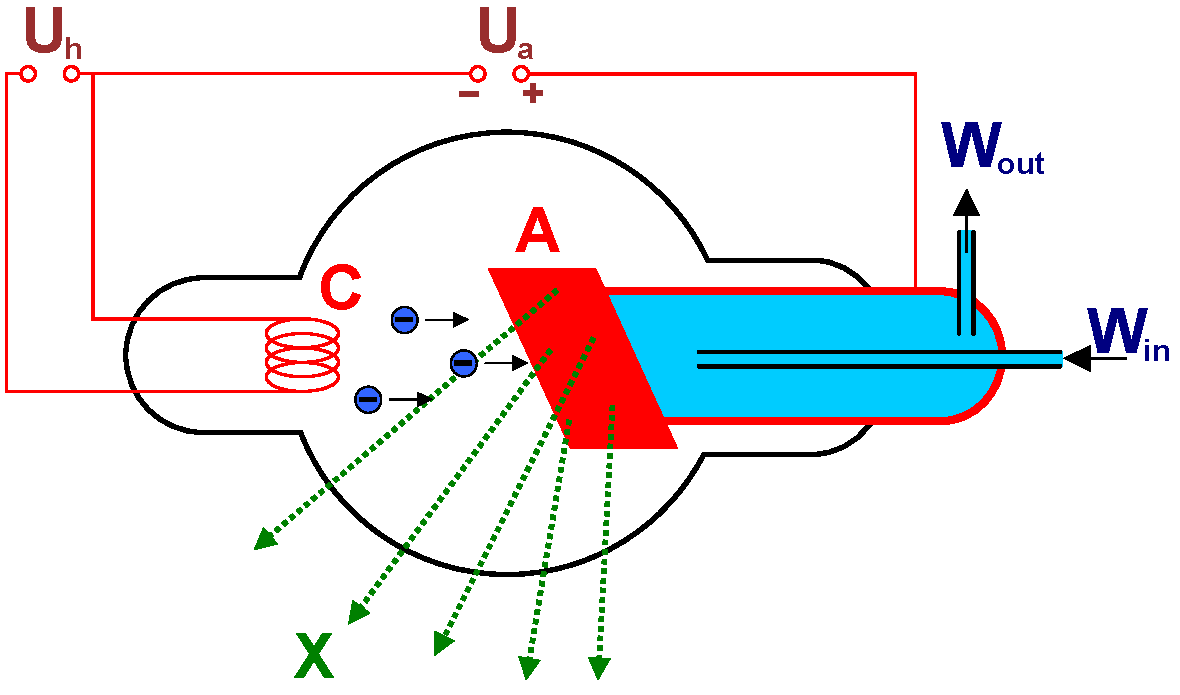
\includegraphics[width=0.5\textwidth]{Abbildungen/WaterCooledXrayTube.pdf}
    \caption{Schematischer Aufbau einer Röntgenröhre nach~\cite{Roentgenroehre}. Da beim Aufprall der Elektronen viel Wärme entsteht, muss die Anode mithilfe eines Wasserzuflusses $W_\text{in}$ gekühlt werden.}
    \label{fig:Roentgenroehre}
\end{figure}\\
Beim Aufschlagen auf die Anode werden die Elektronen abgebremst und strahlen Energie in Form von elektromagnetischen Wellen ab. Idealerweise würde die gesamte kinetische Energie in Röntgenstrahlung umgewandelt werden.
\begin{align}
  e U = E_\text{kin} = h \cdot \nu_\text{max} = \frac{hc}{\lamda_\text{min}}
\end{align}
Allerdings wird ein großer Teil der kinetischen Energie in Wärme umgesetzt, sodass die Anode gekühlt werden muss. Der schematische Aufbau einer Röntgenröhre ist in Abbildung \ref{fig:Roentgenroehre} dargestellt.\\
Das Emissionsspektrum der Anode wird durch ihr Material und der Beschleunigungsspannung der Röntgenröhre bestimmt und setzt sich aus zwei Komponenten zusammen.\\
Die erste Komponente wird \glqq{}weiße Röntgenstrahlung\grqq{} genannt und erscheint allein durch das Abbremsen der Elektronen in der Oberflächenschicht des Targets. Die zweite Komponente bildet die charakteristische Röntgenstrahlung, die normalerweise aus zwei Linien besteht. Hier geschehen Übergänge zwischen den inneren Schalen der Atome des Targets. Gewöhnlich sind die Schalen vollständig mit Elektronen besetzt, jedoch können die hochenergetischen, eingeschossenen Elektronen die gebundenen Elektronen herausschlagen und dort freie Energieniveaus erzeugen. In diese können anschließend Elektronen höherer Niveaus unter Photonenemission übergehen. Diese Linien fester Frequenz werden im Spektrum als K$_\alpha$- bzw. als K$_\beta$-Linien bezeichnet. Das 'K' steht für die Schale, die besetzt wird und der Index beschreibt, aus welcher Schale das Elektron kam, welches den Platz besetzt. Für $\alpha$ handelt es sich um die nächstliegende L-Schale.
% ***** Zwei Bilder nebeneinander *****

% \begin{figure}[htp]
%     \centering
%     \begin{subfigure}{0.45\textwidth}
%         \includegraphics[width=\textwidth]{Bilder/Beispielbild.png}
%     \end{subfigure}
%     \begin{subfigure}{0.45\textwidth}
%         \includegraphics[width=\textwidth]{Bilder/Beispielbild.png}
%     \end{subfigure}
%     \caption{Beschreibung}
% \end{figure}

%***** Tabellen *****
% \begin{table}[ht]
% 	\centering
% 	\caption{Überschrift der Tabelle}
% 	\label{tab:Tabelle1}
% 	\begin{tabular}{l c c c}
% 		\toprule
% 	    text & text & text & text\\
% 	 	\midrule
% 			text & text & text & text\\
% 			text & text & text & text
% 	\end{tabular}
% \end{table}

% *********************************************
% ***** KAPITEL 3 *****************************
% *********************************************
\section{Versuchsdurchführung} \label{sec:Versuchsdurchführung}
Prinzip-Zeichnungen, Versuchsanordnung, Geräte,Vorgehensweise, Schaltpläne.


% *********************************************
% ***** KAPITEL 4 *****************************
% *********************************************
\section{Ergebnisse und Diskussion}
Tabellen mit gemessenen und berechneten Werten, Abbildungen, Diagramme usw. mit Unterschriften sowie Vorgehensweise, Kommentare, Fehlerrechnung.\\
Diskussion der Messergebnisse, Diagramme, Fehlerquellen usw. aus physikalischer Sicht, Vergleich mit der Literatur und theoretischen Werten usw.

% *********************************************
% ***** KAPITEL 4 *****************************
% *********************************************
\section{Zusammenfassung}
Lorem ipsum dolor sit amet, consetetur sadipscing elitr, sed diam nonumy eirmod tempor invidunt ut labore et dolore magna aliquyam erat, sed diam voluptua. At vero eos et accusam et justo duo dolores et ea rebum. Stet clita kasd gubergren, no sea takimata sanctus est Lorem ipsum dolor sit amet. Lorem ipsum dolor sit amet, consetetur sadipscing elitr, sed diam nonumy eirmod tempor invidunt ut labore et dolore magna aliquyam erat, sed diam voluptua. At vero eos et accusam et justo duo dolores et ea rebum. Stet clita kasd gubergren, no sea takimata sanctus est Lorem ipsum dolor sit amet.

% ***** Literaturverzeichnis ******************

\begin{thebibliography}{xxx}
	\bibitem{Demtroeder}
	W. Demtröder: \textit{Experimentalphysik}. Springer Verlag Berlin Heidelberg New York 2008 (5. Auflage).
	\bibitem{Glockner}
	R. Glocker: \textit{Materialprüfung mit Röntgenstrahlen}. Springer Verlag Berlin Heidelberg New York 1985.
  \bibitem{Kleber}
	W. Kleber u.a.: \textit{Einführung in die Kristallographie}. Verlag Technik GmbH 2010 (19. Auflage).
  \bibitem{Roentgenroehre}
  Url: \url{https://commons.wikimedia.org/wiki/File:WaterCooledXrayTube.svg}, (Stand: 20.10.2019)
\end{thebibliography}

\end{document}
